From the given infromation, 
\begin{align}
\vec{A} = \myvec{a/2\\h} = \myvec{4\\4}, \vec{B} = \myvec{0\\0}, \vec{C} = \myvec{8\\0}
\end{align}
which are used to plot the triangle in Fig. \ref{tri/2/fig:tri_SSS_triangle}	
%
\begin{figure}[!ht]
\centering
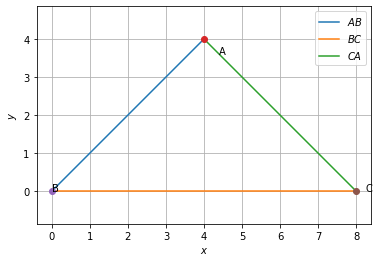
\includegraphics[width=\columnwidth]{solutions/triangle/2/diagram.png}
\caption{isosceles triangle$\triangle ABC$}
\label{tri/2/fig:tri_SSS_triangle}	
\end{figure}


